% Rotate a path around a point: Double Pendulum Case
% https://latexdraw.com
% 13/02/2021, 16:40

\documentclass[border=0.1cm]{standalone}

\usepackage{tikz}

\begin{document}

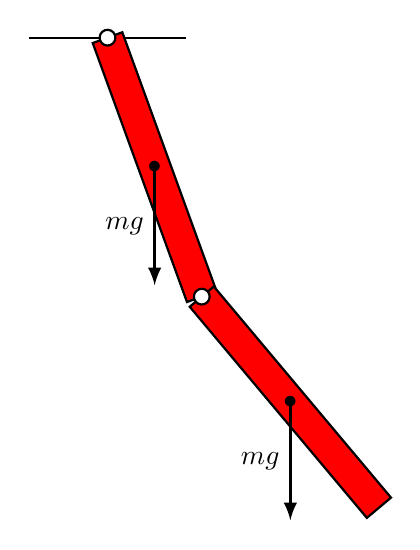
\begin{tikzpicture}[thick]

% Define angles
\newcommand{\angA}{20}
\newcommand{\angB}{20}

% Straight line
\draw (-1,0) -- (1,0);

\begin{scope}[rotate=\angA]

% Pendulum part 1 (red rectangle)
\draw[fill=red] (-0.2,0) rectangle (0.2,-3.5) 
	node[midway](a){$\bullet$};

% Pendulum part 2 (red rectangle)
\draw[fill=red,
	rotate around={\angB:(0,-3.5)}
] (-0.2,-3.5) rectangle (0.2,-7)
	node[midway](b){$\bullet$};

% Two circles filled with white color
\draw[fill=white] (0,-3.5) circle(0.1);
\draw[fill=white] (0,0) circle(0.1);

\end{scope}

% Weight forces
\draw[-latex,very thick] (a.center) -- ++(0,-1.5)
	node[midway,left]{$mg$};
\draw[-latex,very thick] (b.center) -- ++(0,-1.5) 
	node[midway,left]{$mg$};

\end{tikzpicture}

\end{document}
